\chapter{Interactive Document Demo}

\elementbox{intro_text}{\parbox{0.9\textwidth}{\lipsum[1]}}
\narration{intro_text}{First, let's read the introduction. It sets the stage for our topic.}

\begin{figure}[h!]
    \centering
    \elementbox{diagram}{%
    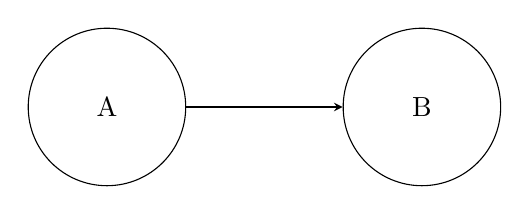
\begin{tikzpicture}
        \node[draw, circle, minimum size=2cm] (A) at (0,0) {A};
        \node[draw, circle, minimum size=2cm] (B) at (4,0) {B};
        \draw[-stealth] (A) -- (B);
    \end{tikzpicture}%
    }
    \caption{A simple diagram.}
\end{figure}
\narration{diagram}{Next, observe this diagram. It shows a transition from state A to state B.}